\section{Appendix}

\subsection{Bib\TeX\ Format} \label{sec:appendixBibTex}
An example Bib\TeX\ entry for work by \citeauthor{BenThesis} \cite{BenThesis}. 
Note, this Bib\TeX\ reference has been formatted with data entries for the AIAA reference format.  

\begin{verbatim}
	@mastersthesis{BenThesis,
		author = {Durante, Benjamin Joseph},
		pages = {1--128},
		school = {University of Calgary]},
		title = {Flying and Handling Qualities of Small-Scale Supersonic Uncrewed Aerial Vehicles},
		note = {{Avaliable: \url{https://dx.doi.org/10.11575/PRISM/40789}}},
		type = {{[Master's} Thesis},
		year = {2023}
	}
\end{verbatim}

\subsection{Figures in \LaTeX} \label{sec:appendixFigureSourceCode}

Figure \ref{fig:mufasaB2} is generated using the following source code:

\begin{verbatim}
	\begin{figure}[hbt!]
		\centering
		\captionsetup{width=0.7\textwidth}
		%\includegraphics[width=0.7\textwidth]{Photos/MUFASA/MUFASA-ISO-Frames-BodyLength.png}
		\def\svgwidth{0.7\textwidth}
		\input{Photos/MUFASA/MUFASA-ISO-Frames-BodyLength.eps_tex}
		\caption{MUFASA B aerodynamic design and coordinate system.}
		%\caption[Short caption for list of figures]{This is the full caption that will appear 
			under the figure.}
		\label{fig:mufasaB2}
		\hfill
	\end{figure}
\end{verbatim}

\subsection{Sub-Figures in \LaTeX} \label{sec:appendixSubFigureSourceCode}

Figure \ref{fig:aircraftComparison} is generated using the following source code:

\begin{verbatim}
	\begin{figure}[hbt!]
		\centering
		\begin{subfigure}{0.48\textwidth}
			\centering
			\captionsetup{width=0.95\linewidth}
			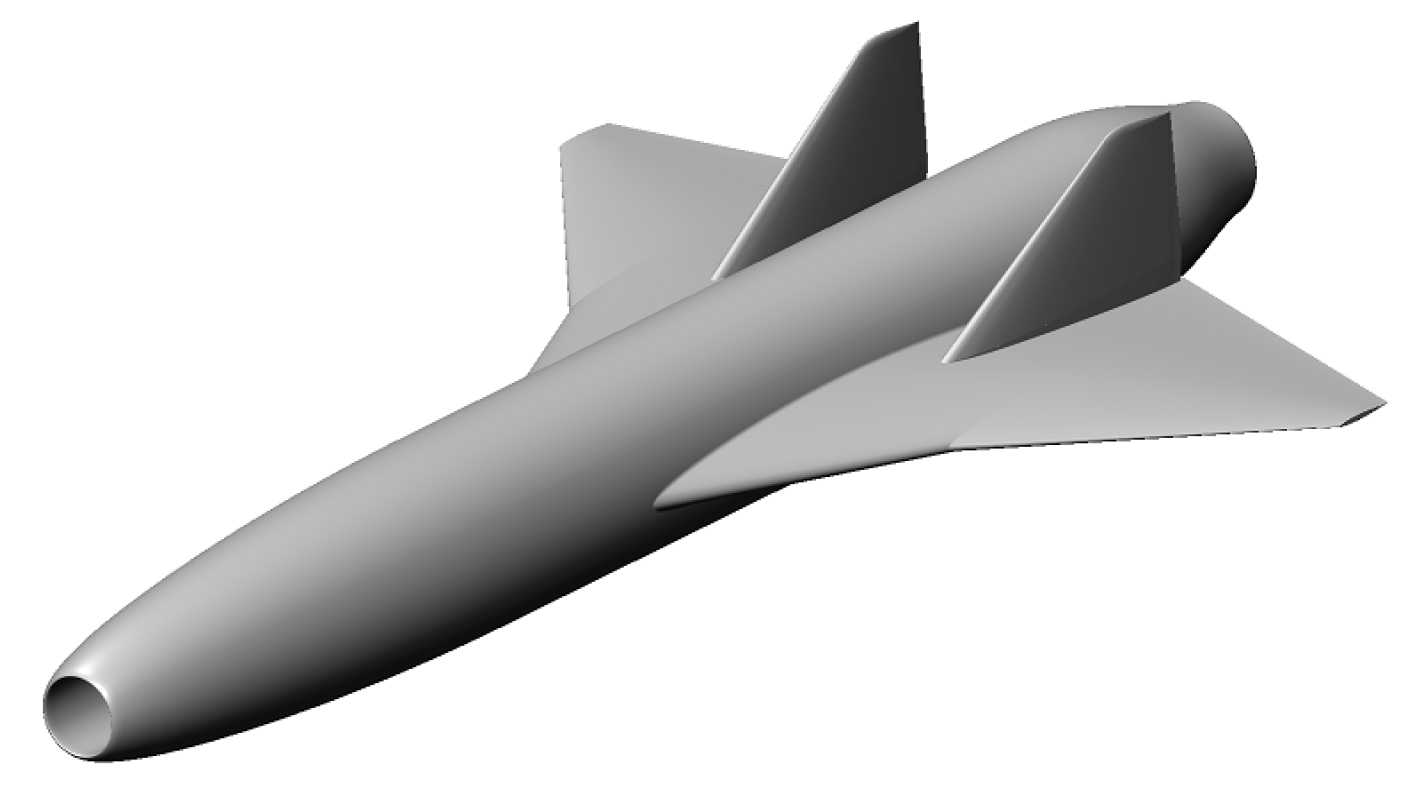
\includegraphics[width=0.95\linewidth]{Photos/Aircraft/MUFASA_Gair}
			\caption{MUFASA A.3, adapted from \citeauthor{ShaunThesis} \cite{ShaunThesis}.}
		\end{subfigure}
		\begin{subfigure}{0.48\textwidth}
			\centering
			\captionsetup{width=0.95\linewidth}
			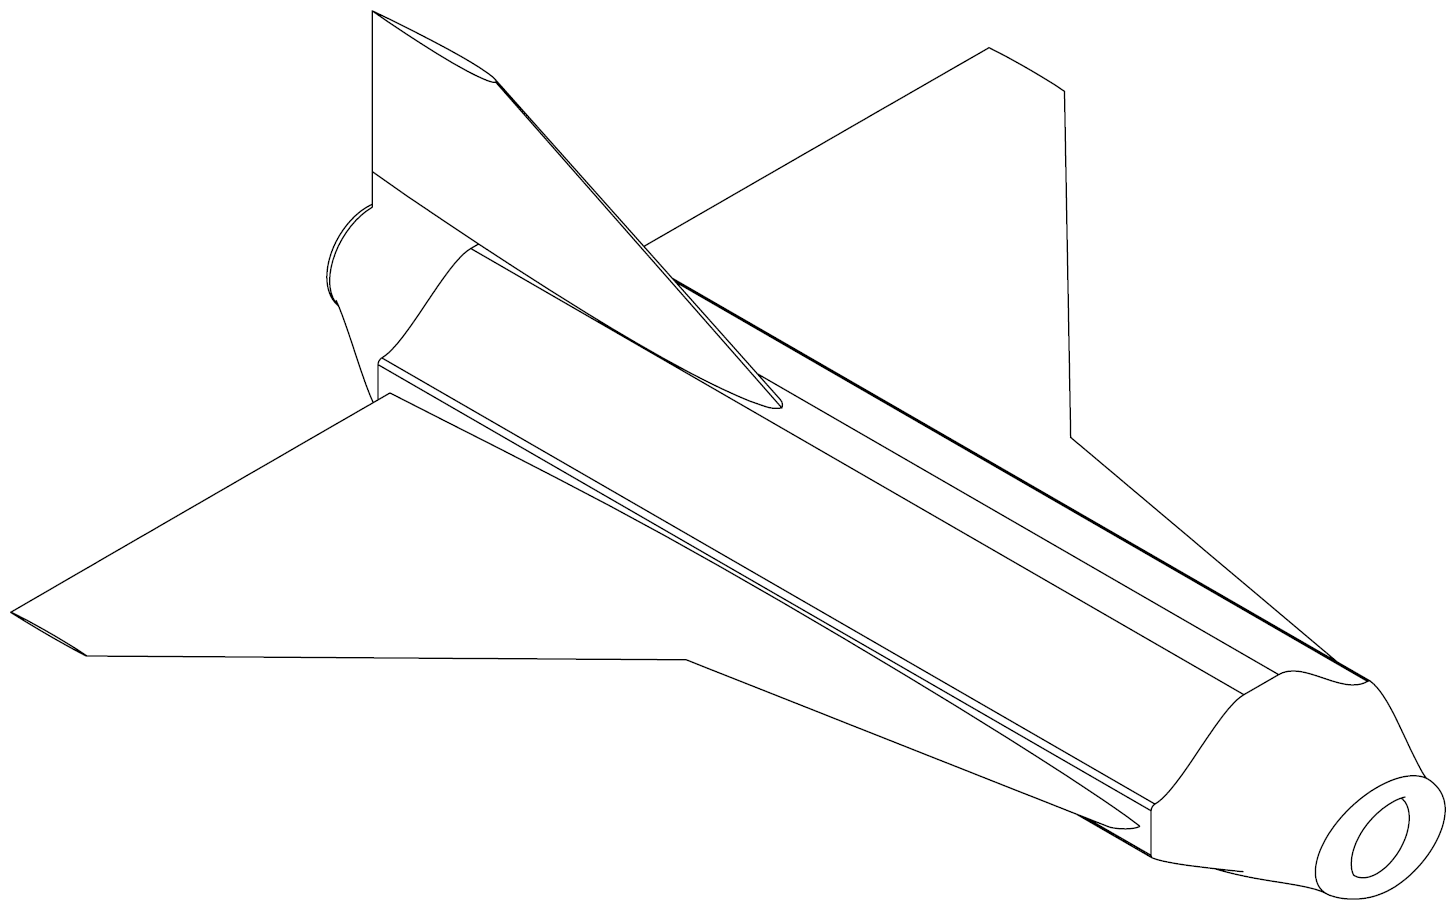
\includegraphics[width=0.95\linewidth]{Photos/Aircraft/MUFASA_ISO}
			\caption{MUFASA B.1.}
		\end{subfigure}
		\caption{MUFASA project aircraft versions (not to scale). \label{fig:aircraftComparison}}
	\end{figure}
\end{verbatim}

\subsection{MATLAB Figure Saving} \label{sec:appendixMatlabFigureCode}

The following MATLAB code automatically saves generated figures. 
The code adjusts the figure text and size, and saves each figure into three file types (.png, .eps, and .svg). 
The code requires that each figure generated has a unique figure name. The figure name from MATLAB is used as the filename, and is extremely useful once multiple result figures are displayed in one document. \cite{LaTeXSymbols}

\lstinputlisting[
frame=single,
numbers=left,
style=Matlab-editor
]{Photos/Code/SaveGeneratedFigures.m}

\subsection{Tables in \LaTeX} \label{sec:appendixTables}

\Cref{tab:tenseBasedOnSection} is generated using the following source code:

\begin{verbatim}
	\begin{table}[hbt!]
		\centering
		\begin{threeparttable}[b]
			\caption{General tense usage in scientific writing sections \cite{tenseScientificWriting}.}
			\label{tab:tenseBasedOnSection}
			\begin{tabular}{cc}
				\toprule
				\textbf{Section} & \textbf{Tense} \\ \midrule
				Abstract & Past \\
				Introduction & Present \\
				Literature Review & Past and Present \\
				Methods & Past \\
				Results & Past \\
				Discussion & Past and Present, and Future \\
				Conclusion & Past, Present, and Future \\ \bottomrule
			\end{tabular}
		\end{threeparttable}
	\end{table}
\end{verbatim}


\subsection{Long Equations in \LaTeX} \label{sec:appendixLongEquation}

Splitting a long equation, as presented in \cref{eqn:dotAngularRateStateExpandedComplete} from \citeauthor{BenThesis} \cite{BenThesis}, is achieved via the code in this section:  

\begin{verbatim}
	\begin{align}
		\begin{split}
			\begin{bmatrix}
				\dot{P} \\
				\dot{Q} \\
				\dot{R}
			\end{bmatrix} &=
			\begin{bmatrix}
				I_{\textup{xx}} & 0 & I_{\textup{xz}} \\
				0 & I_{\textup{yy}} & 0 \\
				I_{\textup{xz}} & 0 & I_{\textup{zz}}
			\end{bmatrix}^{-1}
			\left(
			\left( \left( k_{0} + k_{1} V_{a}^{-2} \right) \delta_{T} S \rho V_{a}^{2} \frac{1}{2}
			\begin{bmatrix}
				1 \\ 0 \\ 0
			\end{bmatrix} \times \left( \bar{r}_{\text{EC}} - \bar{r}_{\text{CG}}\right) +
			\bar{M}_{\textup{aero}} \right) \right. \\
			& \qquad \left. -
			\begin{bmatrix}
				0 & -R & Q \\
				R & 0 & -P \\
				-Q & P & 0
			\end{bmatrix}
			\begin{bmatrix}
				I_{\textup{xx}} & 0 & I_{\textup{xz}} \\
				0 & I_{\textup{yy}} & 0 \\
				I_{\textup{xz}} & 0 & I_{\textup{zz}}
			\end{bmatrix}
			\begin{bmatrix}
				P \\
				Q \\
				R
			\end{bmatrix}
			\right)
		\end{split} \label{eqn:dotAngularRateStateExpandedComplete} 
	\end{align}
\end{verbatim}

\begin{align}
	\begin{split}
		\begin{bmatrix}
			\dot{P} \\
			\dot{Q} \\
			\dot{R}
		\end{bmatrix} &=
		\begin{bmatrix}
			I_{\textup{xx}} & 0 & I_{\textup{xz}} \\
			0 & I_{\textup{yy}} & 0 \\
			I_{\textup{xz}} & 0 & I_{\textup{zz}}
		\end{bmatrix}^{-1}
		\left(
		\left( \left( k_{0} + k_{1} V_{a}^{-2} \right) \delta_{T} S \rho V_{a}^{2} \frac{1}{2}
		\begin{bmatrix}
			1 \\ 0 \\ 0
		\end{bmatrix} \times \left( \bar{r}_{\text{EC}} - \bar{r}_{\text{CG}}\right) + \bar{M}_{\textup{aero}} \right) \right. \\
		& \qquad \left. -
		\begin{bmatrix}
			0 & -R & Q \\
			R & 0 & -P \\
			-Q & P & 0
		\end{bmatrix}
		\begin{bmatrix}
			I_{\textup{xx}} & 0 & I_{\textup{xz}} \\
			0 & I_{\textup{yy}} & 0 \\
			I_{\textup{xz}} & 0 & I_{\textup{zz}}
		\end{bmatrix}
		\begin{bmatrix}
			P \\
			Q \\
			R
		\end{bmatrix}
		\right)
	\end{split} \label{eqn:dotAngularRateStateExpandedComplete} 
\end{align}


% Include PDF shortcut page
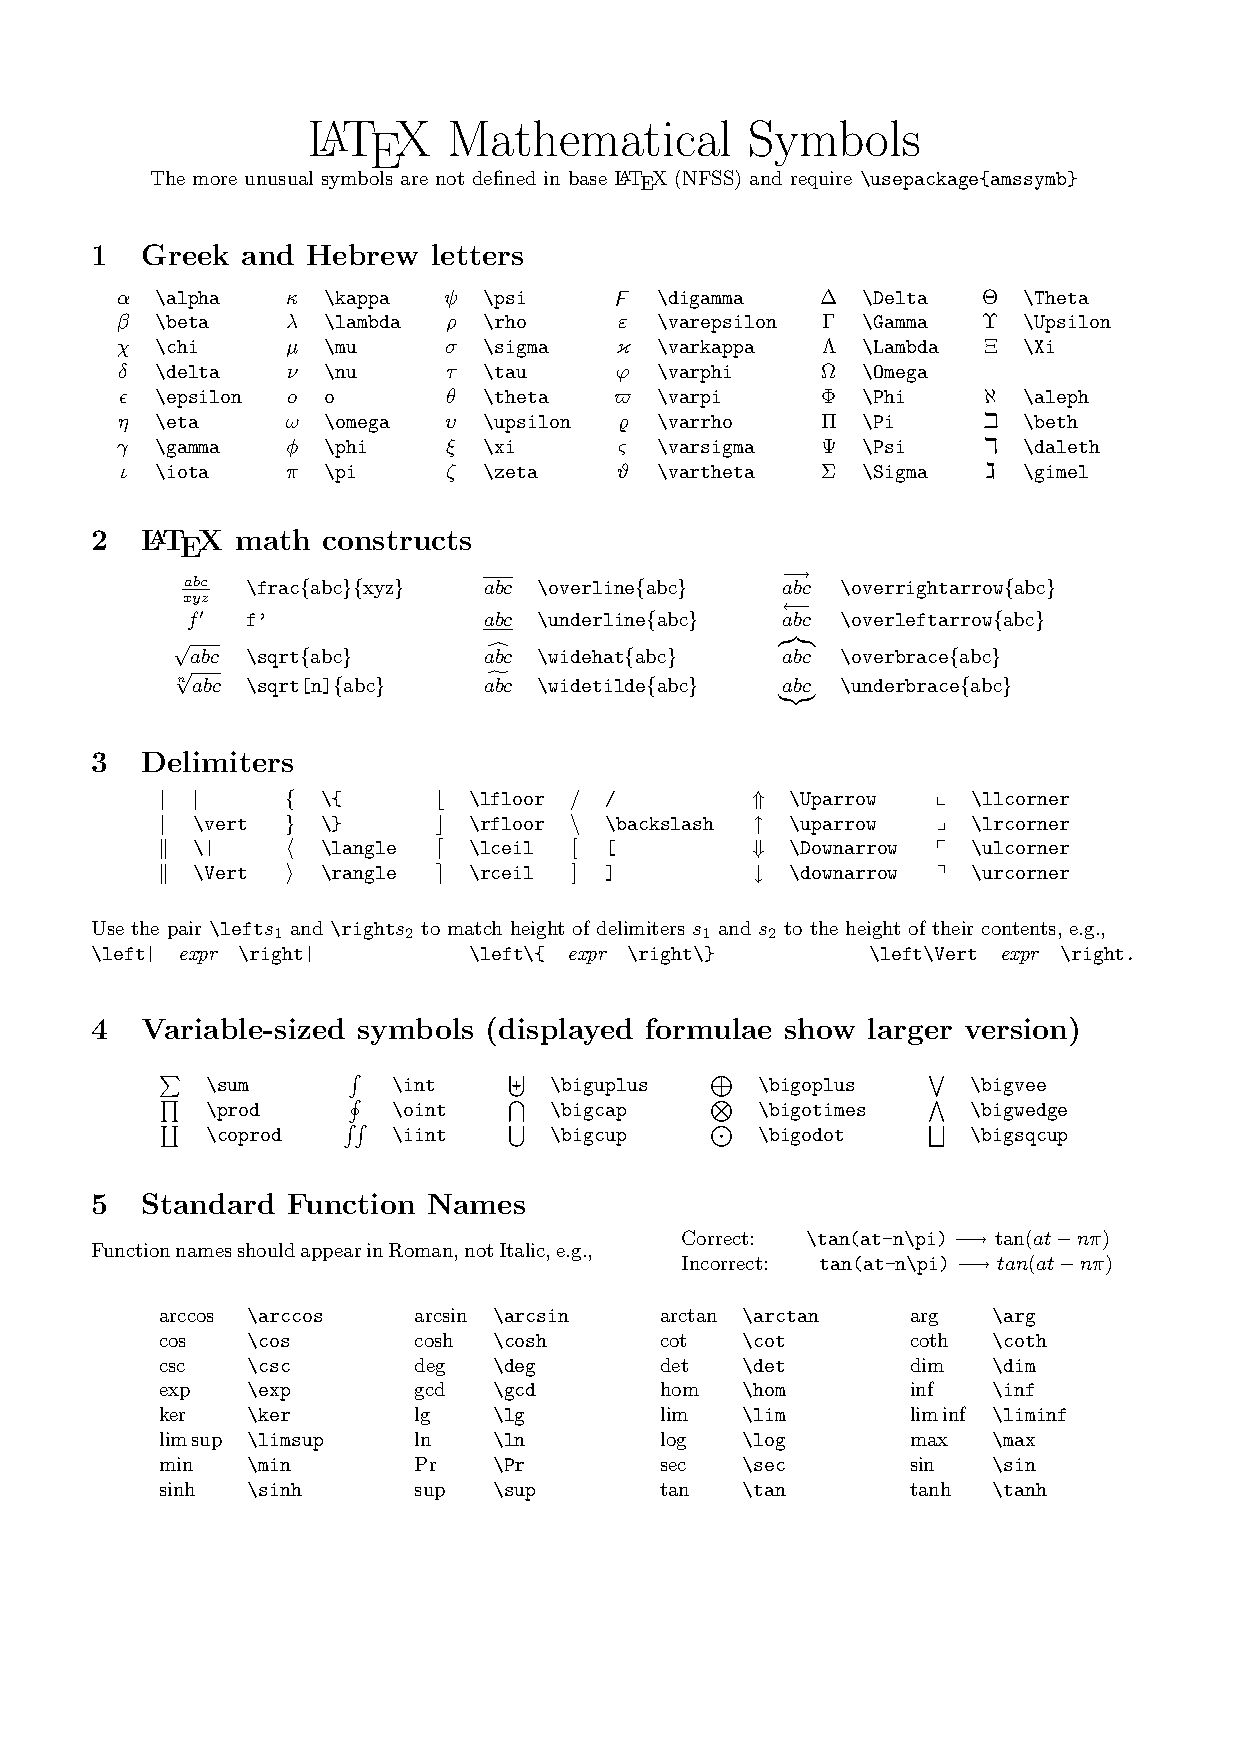
\includepdf[pages=1, pagecommand={\thispagestyle{plain}\subsection{\LaTeX\ Commands} \label{sec:appendixLaTeXSymbols} This section covers common \LaTeX\ commands, reproducing a document created by \citeauthor{LaTeXSymbols} \cite{LaTeXSymbols}.}, width=\linewidth]{Resources/LaTeX-Symbols.pdf}
\includepdf[pages=2-4, pagecommand={\thispagestyle{plain}}, width=\linewidth]{Resources/LaTeX-Symbols.pdf}